\documentclass{article}
\usepackage[utf8]{inputenc}
\usepackage{parskip}
\usepackage{graphicx}
\usepackage{subcaption}
\usepackage{placeins}
\usepackage{geometry}

\title{ANNDA - Lab 2}
\author{Niels Agerskov, Lukas Bjarre, Gabriel Carrizo}
\date{December 2017}

\begin{document}

\maketitle
\pagebreak

\section{Batch Mode Training}

In this part of the lab we trained an RBF network to approximate two functions:

\begin{equation}
  f_1(x) = \sin(2x)
\end{equation}
\begin{equation}
  f_2(x) = \mathrm{square}(2x)
\end{equation}

Where $x \epsilon [0, 2\pi]$ which is sampled with a step sizeof 0.1. The function is consequently tested with $x_{test} = x+0.05$.

\textbf{Try to vary the number of units to get the absolute residual error below 0.1, 0.01 and 0.001 in the residual value (absolute residual error is understood as the average absolute difference between the network outputs and the desirable target values). Please discuss the results, how many units are needed for the aforementioned error thresholds?}

\begin{figure}[ht!]
    \centering
    \begin{subfigure}[t]{0.4\textwidth}
        \centering
        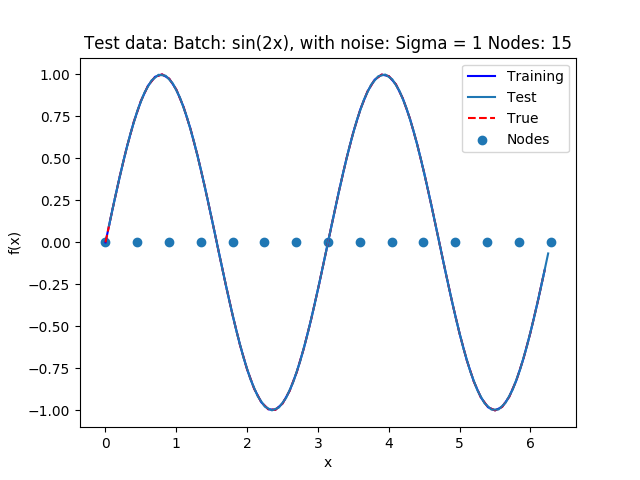
\includegraphics[width=1\textwidth]{plots/batch/best_sin2x.png}
        \caption{}
    \end{subfigure}
    \begin{subfigure}[t]{0.4\textwidth}
        \centering
        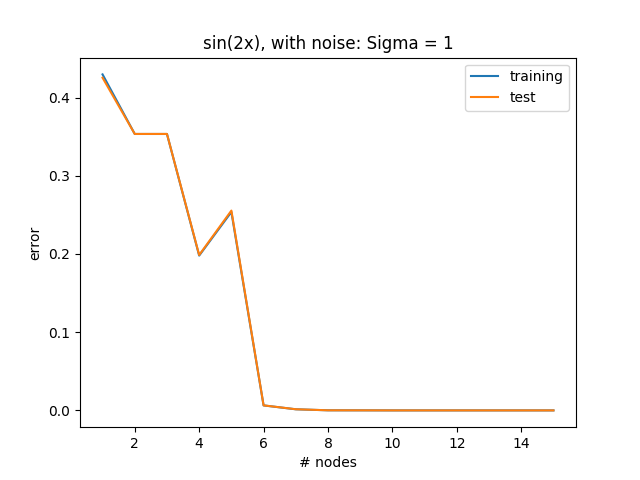
\includegraphics[width=1\textwidth]{plots/batch/best_sin2x_error.png}
        \caption{}
    \end{subfigure}
    \begin{subfigure}[t]{0.4\textwidth}
        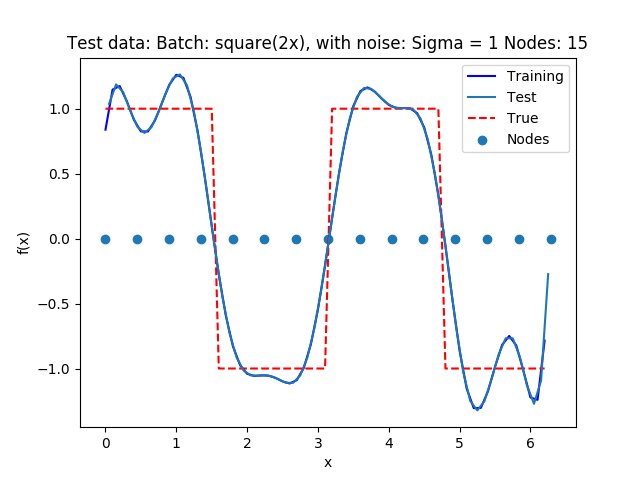
\includegraphics[width=1\textwidth]{plots/batch/best_square2x.png}
        \caption{}
    \end{subfigure}
    \begin{subfigure}[t]{0.4\textwidth}
        \centering
        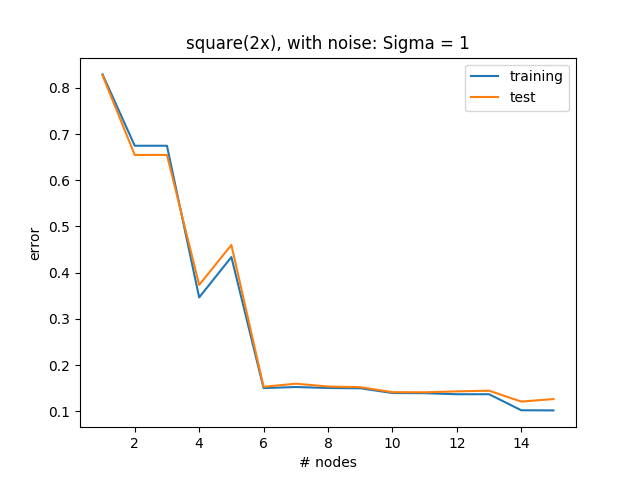
\includegraphics[width=1\textwidth]{plots/batch/best_square2x_error.png}
        \caption{}
    \end{subfigure}
\end{figure}

\begin{figure}[ht!]
  \centering
  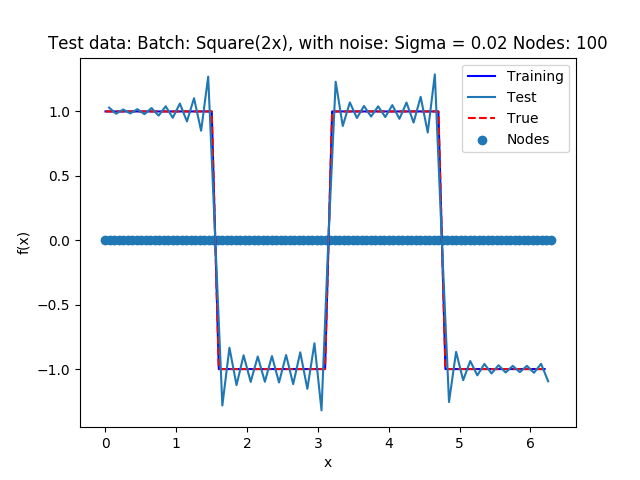
\includegraphics[width=0.5\linewidth]{plots/batch/best_square2x_extreme}
  \caption{test error 0.06}
  \label{}
\end{figure}

\textbf{How can you simply transform the output of your RBF network to re- duce the residual error to 0 for the square(2x) problem? Still, how many units do you need? In what type of applications could this transform be particularly useful?}

The residual error can be reduced to 0 by applying a sign function to the output which will act as a activation function. While this greatly improves the result, about ?? nodes were still necessary. This type of activation is useful when the RBF network should be used as a classifier. 

\begin{figure}[ht!]
    \centering
    \begin{subfigure}[t]{0.4\textwidth}
        \centering
        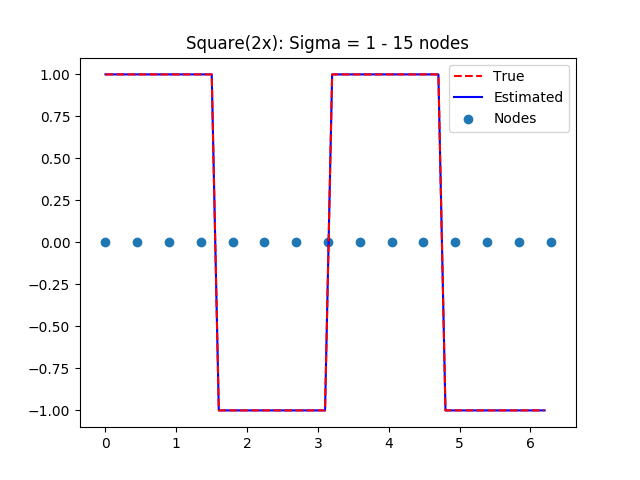
\includegraphics[width=1\textwidth]{plots/batch/best_square_cheat.png}
        \caption{}
    \end{subfigure}
    \begin{subfigure}[t]{0.4\textwidth}
        \centering
        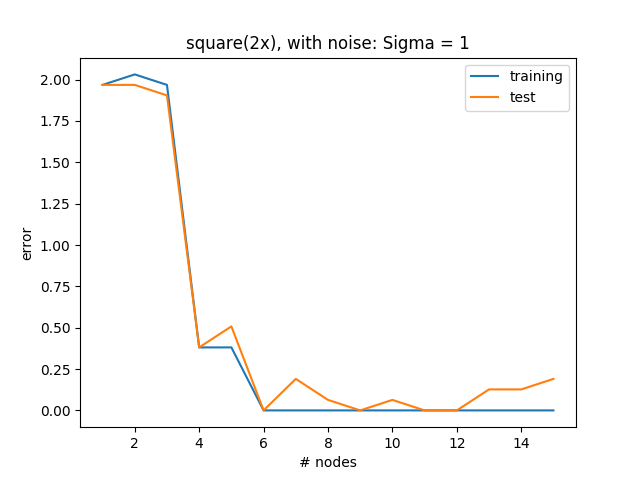
\includegraphics[width=1\textwidth]{plots/batch/square_error_sign}
        \caption{}
    \end{subfigure}
    \caption{Taking the sign of the estimated square function makes us reach 0 error with only 6 nodes.}
\end{figure}

\section{Regression with noise}
\FloatBarrier
Effect of altering sigma:
\FloatBarrier
\begin{figure}[ht!]
    \centering
    \begin{subfigure}[t]{0.4\textwidth}
        \centering
        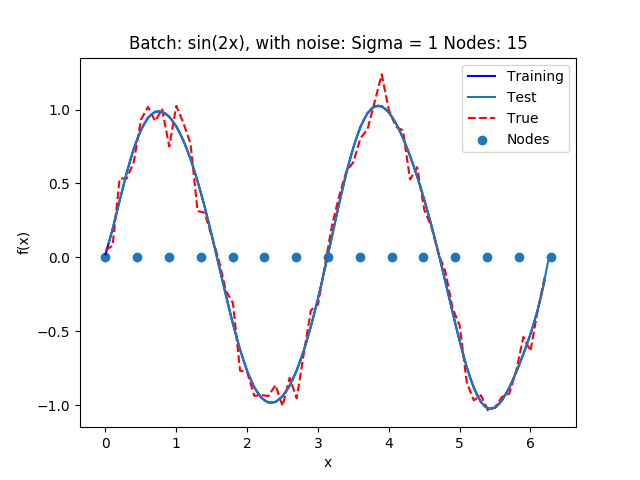
\includegraphics[width=1\textwidth]{plots/noise/batch_sin2x_sigma1.png}
        \caption{}
    \end{subfigure}
    \begin{subfigure}[t]{0.4\textwidth}
        \centering
        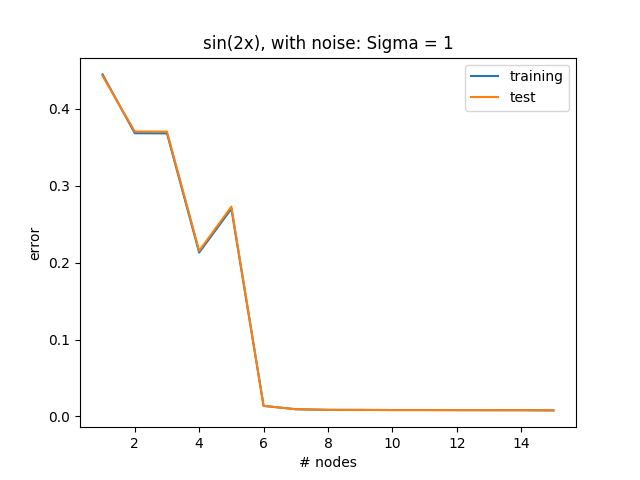
\includegraphics[width=1\textwidth]{plots/noise/batch_sin2x_error_sigma1.png}
        \caption{}
    \end{subfigure}
    \begin{subfigure}[t]{0.4\textwidth}
        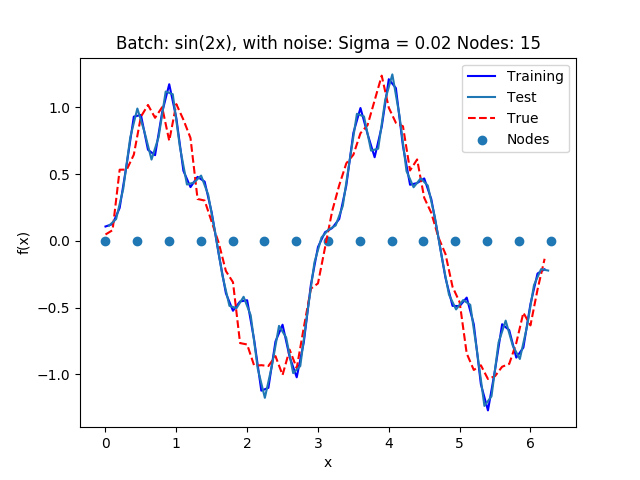
\includegraphics[width=1\textwidth]{plots/noise/batch_sin2x_sigma_002}
        \caption{}
    \end{subfigure}
    \begin{subfigure}[t]{0.4\textwidth}
        \centering
        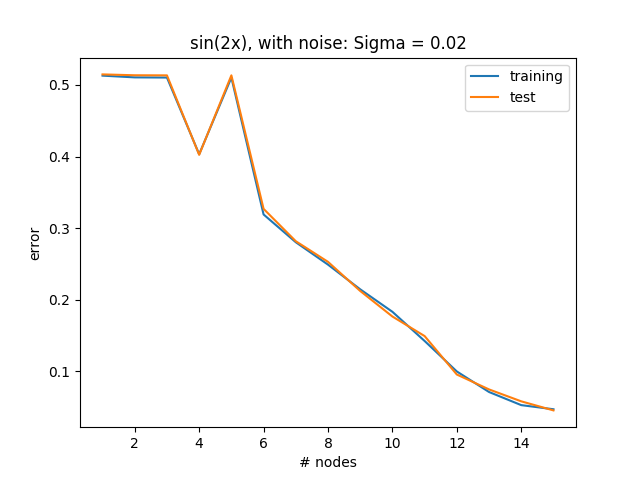
\includegraphics[width=1\textwidth]{plots/noise/batch_sin2x_error_sigma_002}
        \caption{}
    \end{subfigure}
    \caption{Plots of the effect of altering sigma on networks trained with batch method}
\end{figure}


\begin{figure}[ht!]
    \centering
    \begin{subfigure}[t]{0.4\textwidth}
        \centering
        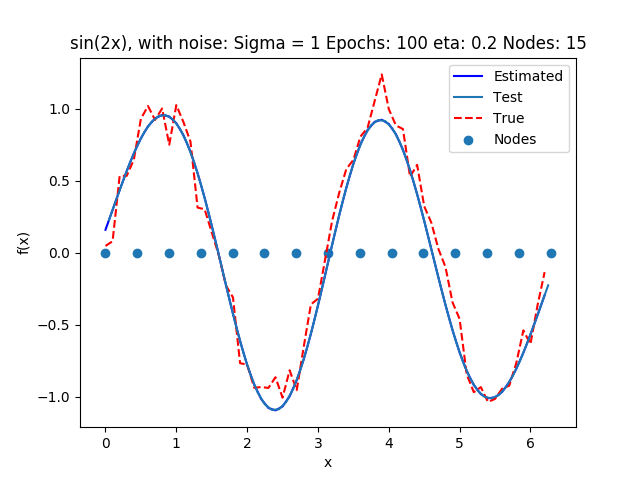
\includegraphics[width=1\textwidth]{plots/noise/seq_sin2x_100ep_sigma1}
        \caption{}
    \end{subfigure}
    \begin{subfigure}[t]{0.4\textwidth}
        \centering
        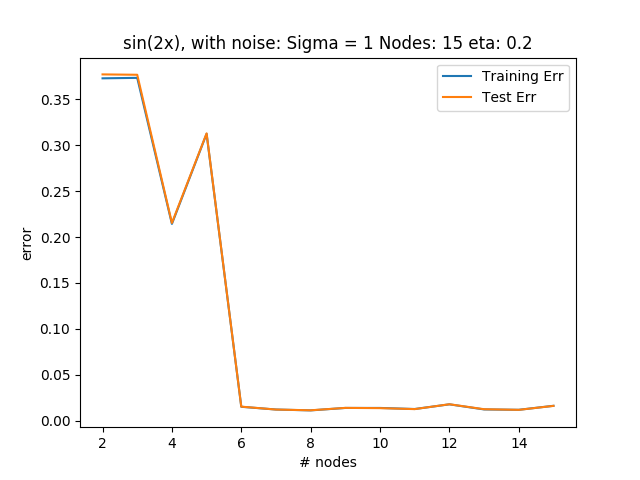
\includegraphics[width=1\textwidth]{plots/noise/seq_sin2x_100ep_sigma1_error}
        \caption{}
    \end{subfigure}
    \begin{subfigure}[t]{0.4\textwidth}
        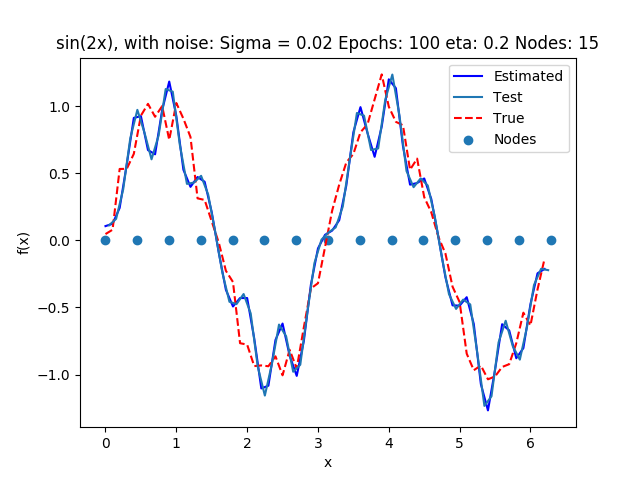
\includegraphics[width=1\textwidth]{plots/noise/seq_sin2x_100ep_sigma002}
        \caption{}
    \end{subfigure}
    \begin{subfigure}[t]{0.4\textwidth}
        \centering
        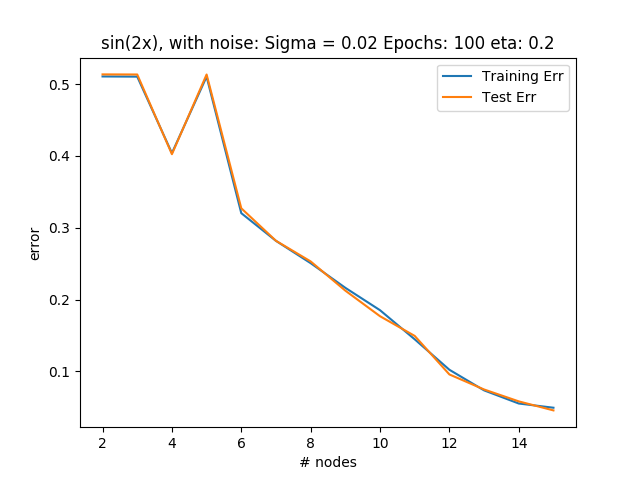
\includegraphics[width=1\textwidth]{plots/noise/seq_sin2x_100ep_sigma002_error}
        \caption{}
    \end{subfigure}
    \caption{Plots of the effect of altering sigma on networks trained with sequential method}
\end{figure}

Effect of number of epochs:

\begin{figure}[ht!]
    \centering
    \begin{subfigure}[t]{0.4\textwidth}
        \centering
        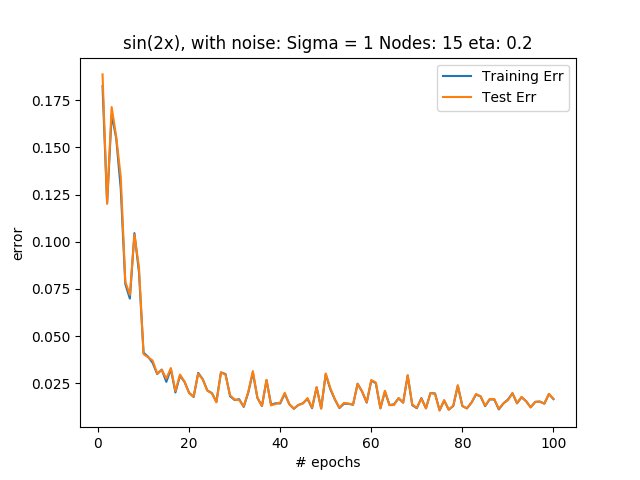
\includegraphics[width=1\textwidth]{plots/noise/seq_sin2x_15nodes_sigma1_error_per_epoch.png}
        \caption{}
    \end{subfigure}
    \begin{subfigure}[t]{0.4\textwidth}
        \centering
        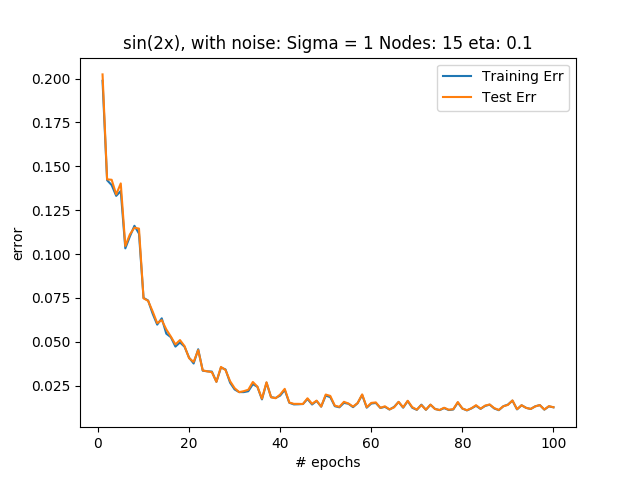
\includegraphics[width=1\textwidth]{plots/noise/seq_sin2x_15nodes_sigma1_error_per_epoch_eta01.png}
        \caption{}
    \end{subfigure}
    \begin{subfigure}[t]{0.4\textwidth}
        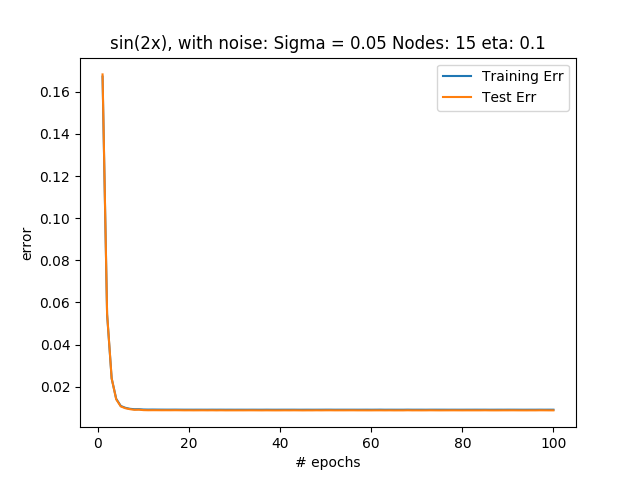
\includegraphics[width=1\textwidth]{plots/noise/seq_sin2x_15nodes_sigma1_error_per_epoch_eta005.png}
        \caption{}
    \end{subfigure}
    \begin{subfigure}[t]{0.4\textwidth}
        \centering
        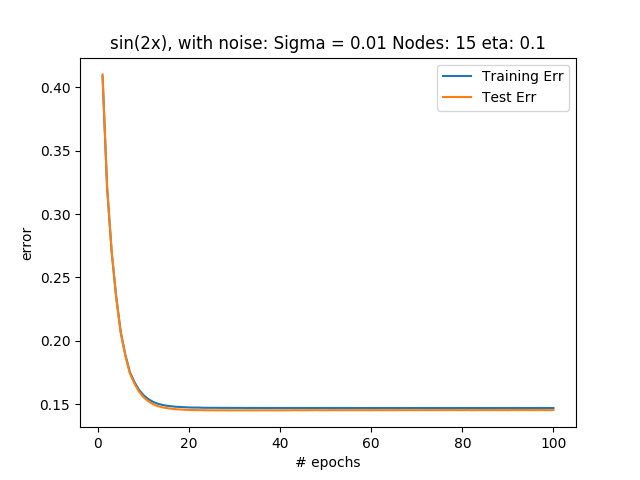
\includegraphics[width=1\textwidth]{plots/noise/seq_sin2x_15nodes_sigma1_error_per_epoch_eta001.png}
        \caption{}
    \end{subfigure}
    \caption{Plots of the error as a function of eta on networks trained with sequential method}
\end{figure}

The positioning of nodes in the input space is quite important. The strategy used was to place the nodes at even intervals of quarter pi, aiming to place the nodes at the tops and bottoms of the sinus wave. This method was better than totally random placement since the shape of the RBF functions approximate the shape of the tops and bottoms of the sinus wave quite well. 

Changing the width of the RBF functions changed the amount of smoothing applied to the input data. A larger width resulted in a smoother prediction, more similar to the underlying function. A smaller width resulted in a prediction containing more of the noise that was added to the labels.

In comparison to a MLP network the RBF approach is way more efficient and accurate at predicting the sinus function. This was especially noticeable when it came to prediction of validation data where it was impossible to predict any of the function noise. The training time was also magnitudes higher with at least 15000 epochs was necessary to approach convergence.

\section{Competitive Learning}

\begin{figure}[ht!]
    \centering
    \begin{subfigure}[t]{0.4\textwidth}
        \centering
        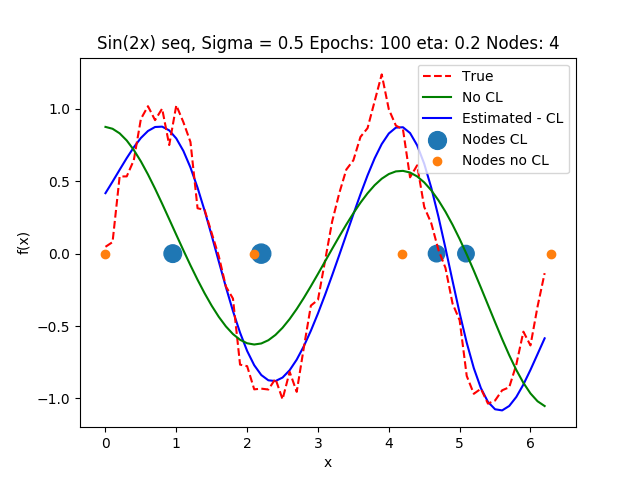
\includegraphics[width=1\textwidth]{plots/cl/sin2x_seq_CL_vs_no_cl_plots}
        \caption{Generated functions plotted with the node RBF node positions, with and without CL.}
    \end{subfigure}
    \begin{subfigure}[t]{0.4\textwidth}
        \centering
        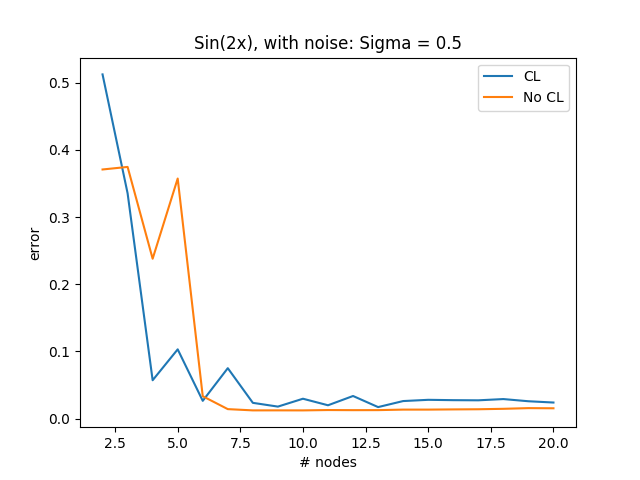
\includegraphics[width=1\textwidth]{plots/cl/sin2x_seq_CL_vs_no_cl_plots_error}
        \caption{Error as a function of the number of nodes, with and without competitive learning.}
    \end{subfigure}
    \caption{Plots of the effects of Cmpetitive Learning}
\end{figure}

\begin{figure}[ht!]
    \centering
    \begin{subfigure}[t]{0.4\textwidth}
        \centering
        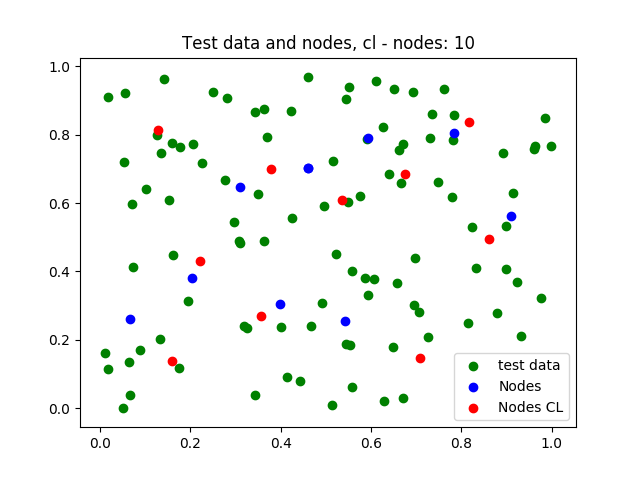
\includegraphics[width=1\textwidth]{plots/2d/input_basic_both_cl_batch_test}
        \caption{Test data and the node positions before and after competitive learning}
    \end{subfigure}
    \begin{subfigure}[t]{0.4\textwidth}
        \centering
        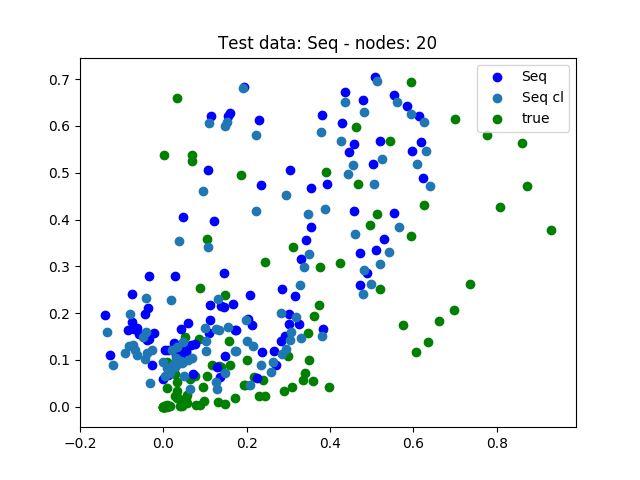
\includegraphics[width=1\textwidth]{plots/2d/first_basic_both_CL_output_seq_test_20_sigma25}
        \caption{Output of networks trained with and without competitive learning}
    \end{subfigure}
    \caption{}
\end{figure}

<<<<<<< HEAD
The effects of applying competitive learning were quite weak. The resulting predictions could be improved a bit which can be seen in the result plots. Perhaps more interesting is what hap pend to the location of the nodes in the input space. The nodes were noticeably more spread out, allowing for better representation of the input data. There were still some areas near the middle of the data where multiple nodes ended up, however at the edges the nodes placed with the use of CL reached much more of the input data. The same amount of "representation" could probably have been reached with random placement, however with CL this could be done using a lot fewer nodes.

\FloatBarrier
\section{Topological Ordering of Animals}
As can be seen in the plot, similar animals are grouped together. This is expected due to how the weight nodes are aggregated together using neighbourhoods. The neighbourhood is defined with a cutoff at the edges, so index 0 and index N, where N is the maximum index are considered far away from each other. One interesting observation is that bat and elephant end up very close together. While this might seem wrong, if the distance between their respective attribute vectors are computed they end up at a distance of about 3 from each other. This is quite close considering that the minimum distance is about 1.6 and the maximum distance is about 5.6.

% PLOT OF ANIMAL ORDER

\section{Cyclic Tour}
In this part  a similar network as in the last part was created, with the main difference being that the neighbourhood is now cyclic so that the first and last index are considered neighbours. Most of the time the network is able to find a short route however it sometimes get stuck in a local minimum and has to cross over another path. This is most likely due to the stochastic nature of how the weights are initiated. 

% PLOT OF GOOD AND BAD CYCLIC TOUR

\section{Data Clustering: Votes of MPs}
In this part the 31-dimensional input data consisting of how different MPs of parliament cast their votes in 31 different questions was mapped to a 10x10 grid, visualising voting patterns. These patterns were then evaluated with respect to gender, district and party alignment. In both the gender and party alignment obvious trends could be observed. Most of the time MPs belonging to parties with similar political alignments would place their votes in the same quadrant, while MPs of opposite parties would be spread apart. When evaluated with respect to gender it was easy to see that MPs voted very similarly independent of being male or female. Finally for the district evaluation it was hard to draw any conclusions other than that vote patterns were heavily dependant on the size of the districts. Bigger districts had a larger spread in their votes than smaller districts.

% PLOT OF PARTY VOTES

% PLOT OF GENDER VOTES

% PLOT OF DISTRICT VOTES
=======
>>>>>>> ff6f1e19faa9f9c5d00803d15b4a036b9093652d
\end{document}
